\section{Question 1 à 3}
\begin{figure}[h]
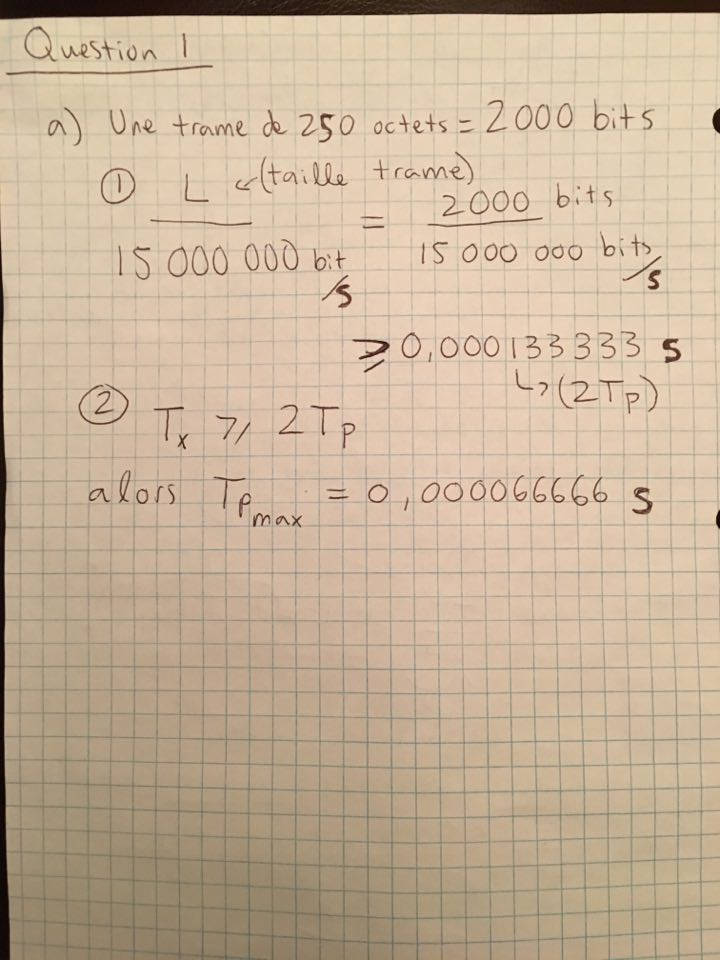
\includegraphics[scale=0.7]{1-1.jpg}
\end{figure}
\begin{figure}[h]
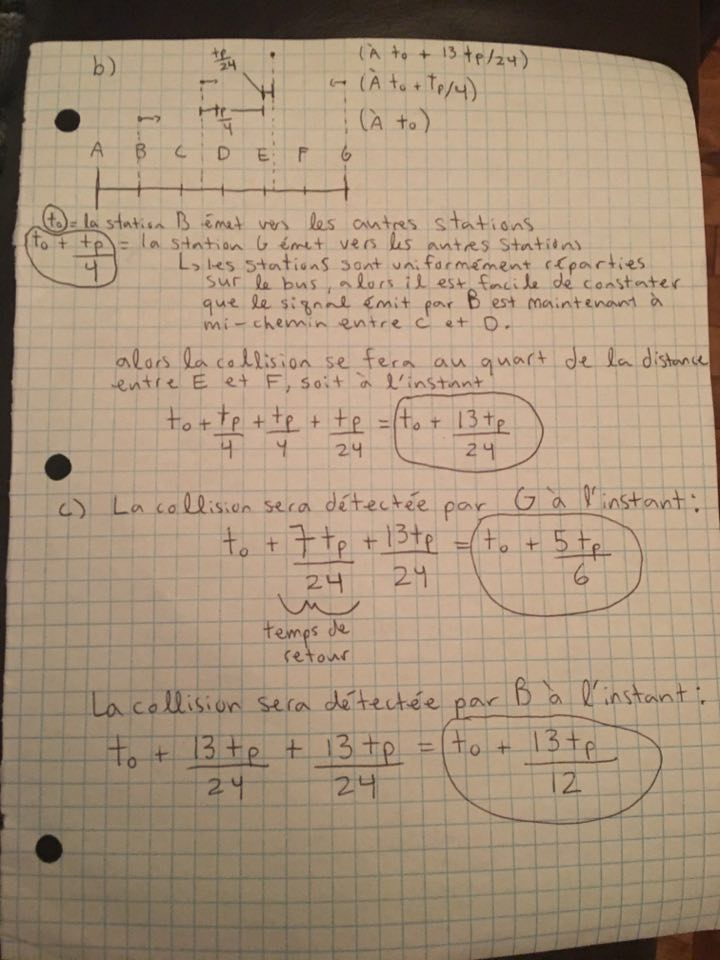
\includegraphics[scale=0.7]{1-2.jpg}
\end{figure}
\begin{figure}[h]
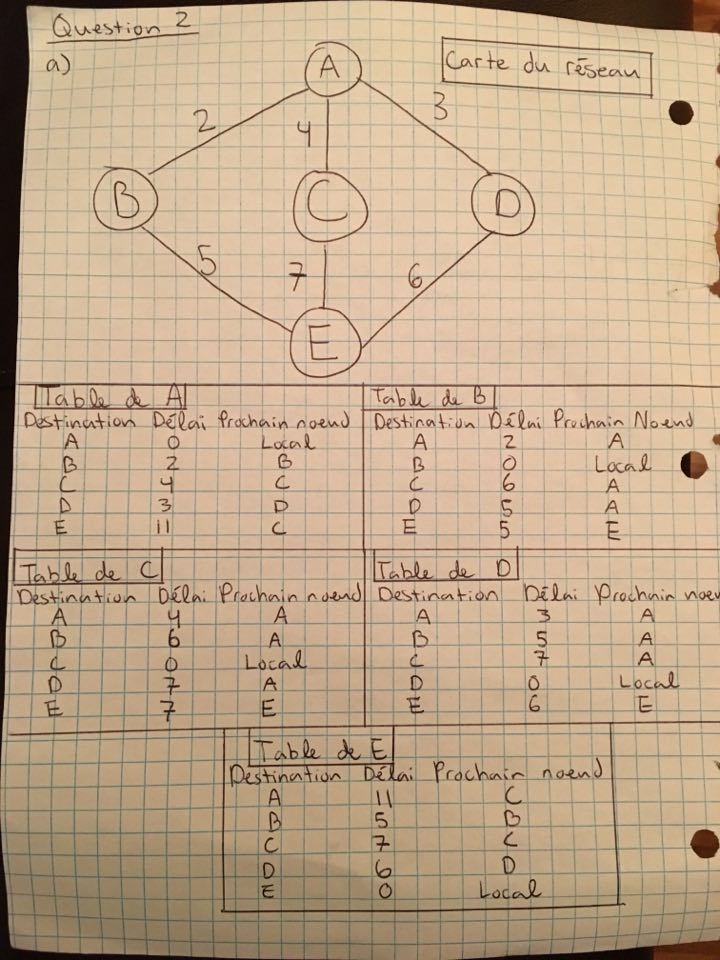
\includegraphics[scale=0.7]{2-1.jpg}
\end{figure}
\begin{figure}[h]
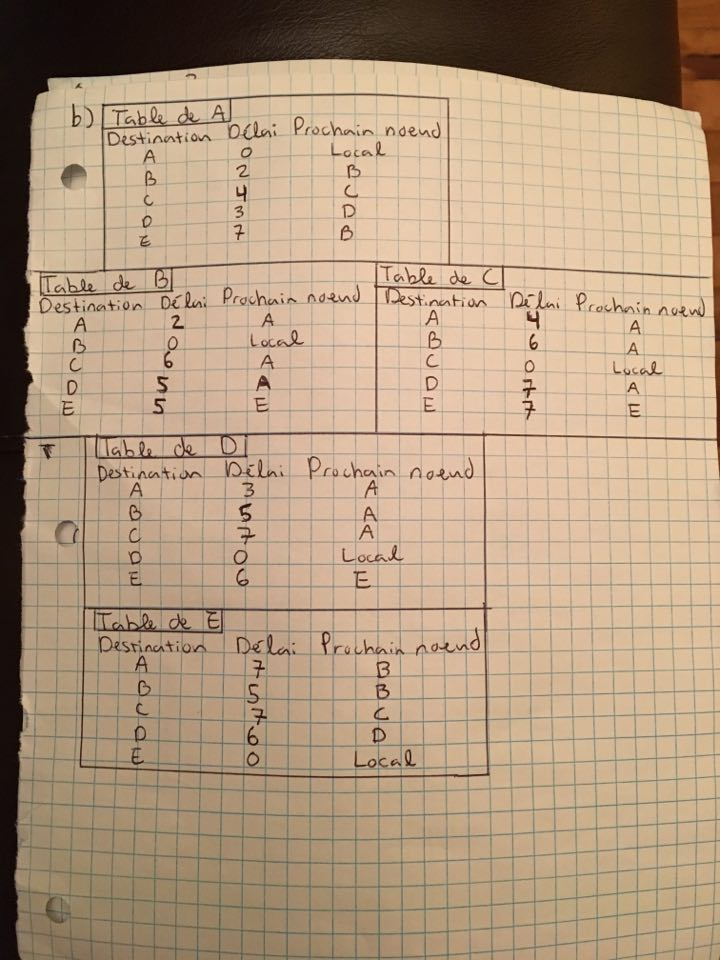
\includegraphics[scale=0.7]{2-2.jpg}
\end{figure}
\begin{figure}[h]
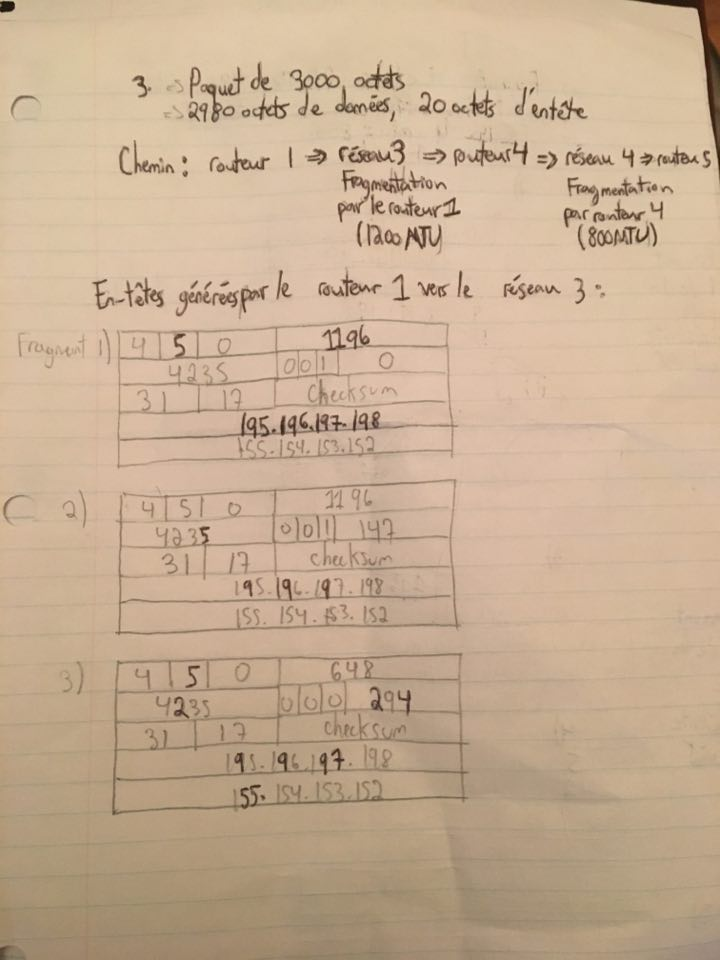
\includegraphics[scale=0.7]{3-1.jpg}
\end{figure}\begin{figure}[h]
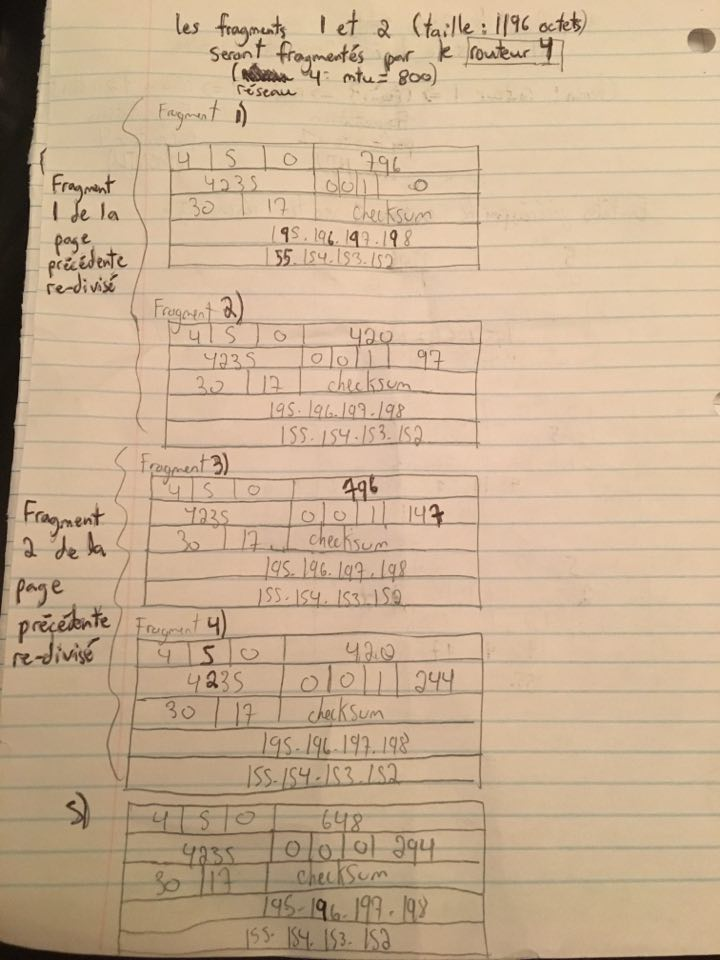
\includegraphics[scale=0.7]{3-2.jpg}
\end{figure}\begin{figure}[h]
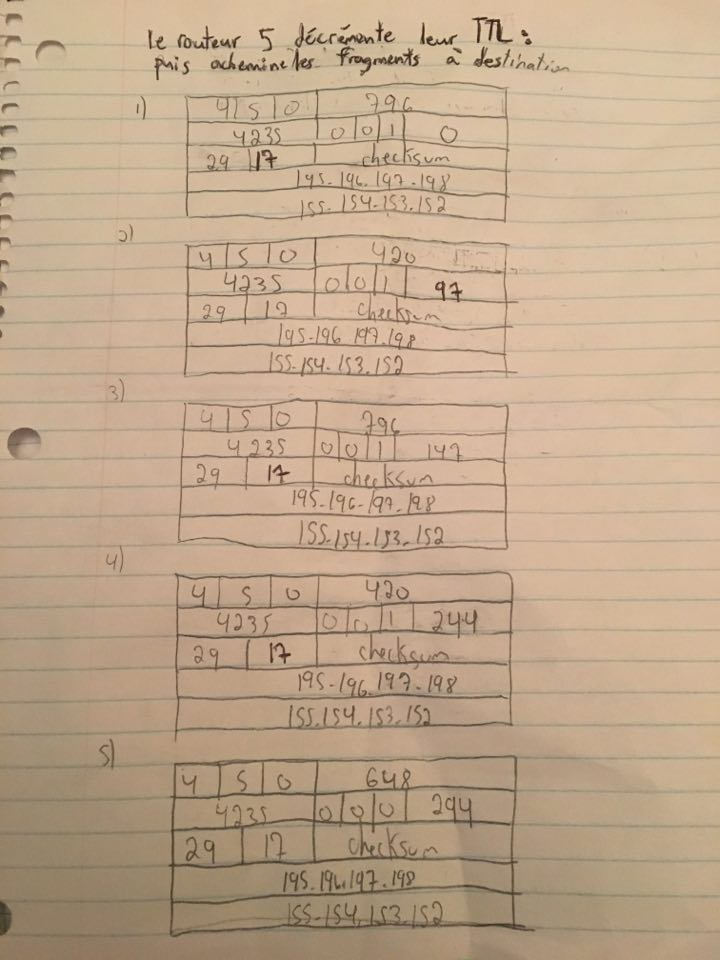
\includegraphics[scale=0.7]{3-3.jpg}
\end{figure}
\clearpage
\section{Question 4}
\begin{enumerate}[(a)]
	\item C'est une réseau de classe 'b' avec masque de sous réseau 
		par defaut : 255.255.0.0
	\item 255.255.254.0
	\item 138.123.0.0, 138.123.2.0, 138.123.4.0
	\item 138.123.250.0, 138.123.252.0, 138.123.254.0
	\item 138.123.10.0, 138.123.10.1, 138.123.10.2
	\item 138.123.10.253, 138.123.10.254, 138.123.10.255
\end{enumerate}

